% 第 4 章 模型管理场景
\chapter{模型管理场景}

\begin{quote}
\textbf{本章范围声明}：EdgeFlow \textbf{v0.7.0（2026-08-25 发布）起内置模型仓库与灰度发布平台}——模型仓库 = 模型 + 版本两级台账 + 部署影子；灰度发布 = 按节点白名单/按比例、分批、fail-fast、取消、回滚（手册 F41/F42 \textbf{已实现}）。模型以“镜像即模型、Tag 即版本”方式纳入平台化台账管理；\textbf{镜像实体仍在客户既有镜像仓库}（平台登记镜像 ref + sha256 摘要，不做镜像上传/分发）；训练平台不在产品范围内。本章 4.2--4.4 为正式能力，4.5 保留 v0.1.0 时代的过渡路径为“兼容路径”小节（仍可用；平台化能力落地后建议切换）。
\end{quote}

\section{业务痛点}

\begin{itemize}
  \item \textbf{模型分发靠人工}：模型文件与运行环境依赖人工拷贝、登录边缘节点手动部署，节点数量一多便不可持续，且极易因人工操作引入错误。
  \item \textbf{版本混乱}：模型缺少统一的版本标识与台账，边缘节点“实际跑的是哪个版本”说不清，出现问题难以定位。
  \item \textbf{边缘更新难}：边缘节点分布广、网络条件不一，逐个节点升级模型成本高、耗时长，更新窗口难以控制。
  \item \textbf{回滚无保障}：升级失败后缺少可靠的版本回退手段，业务长时间中断风险高，运维人员不敢轻易升级。
\end{itemize}

\section{方案设计（平台化正式能力，v0.7.0）}

\textbf{设计定位}：EdgeFlow 云端内置模型仓库与灰度发布能力（F41/F42 已实现，API 契约见产品文档 API-SPEC §7）——模型管理由“镜像 Tag + 手工台账”升级为\textbf{平台化两级台账 + 受控发布流程}；发布/回滚经既有 podsync/config-sync 幂等下发链路到达边缘，\textbf{边缘零代码改动}（旧版 edgecore 直接可用）。

\textbf{模型仓库与版本管理（F41）}：

\begin{itemize}
  \item \textbf{模型台账（Model）}：模型名唯一（字符集白名单，禁 `/`），描述/类型/扩展元数据；\texttt{DELETE} 前置（无 active 版本、无在途发布），级联删除 draft/archived 版本与部署影子。
  \item \textbf{版本台账（ModelVersion）}：“Tag 即版本”——镜像 ref（\textbf{必带 tag}）+ sha256 摘要登记（防篡改，与 F39/F15 镜像完整性语义衔接）+ 架构白名单（amd64/arm64，F38）+ 参数元数据（发布时随版本平铺下发）；版本状态机 \texttt{draft $\rightarrow$ active $\rightarrow$ archived}（activate 自动降级旧 active；archived 可删除、不可再激活；发布/回滚不改变版本状态）。
  \item \textbf{部署影子（F41 台账）}：\seqsplit{\texttt{GET /api/v1/models/\{model\}/deployments}} 提供“版本—节点—时间”追踪；podsync+config-sync 双 acked 后写穿（云端期望态，与边缘实际运行版本分离；重启后 etcd 恢复）。
\end{itemize}

\textbf{模型灰度发布（F42）}：

\begin{itemize}
  \item \textbf{目标选择}：按节点白名单（全部须已注册，422 列出未知节点）/ 按比例（\textbf{分母 = 创建时刻 Ready 节点}，n = ceil(分母 × 百分比 / 100) 上取整，字典序取前 n；0 台 Ready $\rightarrow$ 422）；目标集合\textbf{创建时物化快照}，运行期不重算；不同模式/迁移后的百分比目标集合不跨模式可比（以创建时快照为准）。
  \item \textbf{分批推进}：\texttt{batchSize}（每批节点数，批内逐节点\textbf{串行}——控制批粒度/暂停节奏，非并发度）+ \texttt{pauseBetween} 批间暂停 + \texttt{failFast}（默认开，单节点失败立即中止，剩余节点标 skipped）。
  \item \textbf{取消与回滚}：取消在批次边界生效（剩余节点 ≤1 扫描周期补 skipped）；回滚 = \textbf{逆序批量}执行到 prevActive（批间不暂停），失败不回滚中止（能回多少回多少，perNode 明细可查）；回滚前置守卫：无 prevActive $\rightarrow$ 422；\textbf{已被更新版本接管 $\rightarrow$ 409}（先显式 activate 目标旧版本或发起新发布）。
  \item \textbf{可靠性}：模型/版本/发布等全部 etcd 持久化（写穿 + CAS；纯内存模式任务重启丢失，明示）；同模型在途发布互斥（guard）；外部多副本下 release 级\textbf{领跑锁}与崩溃接管（≤TTL 续跑）。
\end{itemize}

\textbf{下发链路（边缘零改动）}：发布 = 逐节点 podsync（镜像 Pod，命名 \seqsplit{\texttt{edgeflow-model-<sanitized>}}，namespace \texttt{edgeflow}）+ config-sync（ConfigMap：保留键 model/version/mirror/sha256/type/releasedAt + 版本参数平铺）$\rightarrow$ 双 acked 后写穿部署影子 $\rightarrow$ 边缘 MetaManager SQLite 落盘、Edged 声明式收敛、推理容器挂载 ConfigMap 即得“当前模型版本与参数”。回滚同通道把 version 改回 prevActive。

\section{产品特性引用}

\textbf{表 4-1：模型管理场景特性引用}

{\small\setlength{\tabcolsep}{3pt}
\begin{tabular}{@{}p{1.6cm}p{0.8cm}p{3.4cm}p{8.8cm}@{}}
\toprule
环节 & F 编号 & 产品能力 & 说明\\
\midrule
模型台账 & F41 & 模型仓库与版本管理（\textbf{v0.7.0 已实现}） & 云端模型/版本/发布/部署影子台账：17 个新 REST 端点（模型 5 + 版本 6 + 发布 5 + 部署影子 1，\textbf{总端点 14$\rightarrow$31}）；etcd 持久化（纯内存/embed/外部 三模式）\\
灰度发布 & F42 & 模型灰度发布（\textbf{v0.7.0 已实现}） & 白名单/按比例、分批、fail-fast、取消、逆序回滚；服务端调度 + 逐节点结果台账化；命令与节奏建议见 4.4\\
声明下发 & F31 & 云端 API 下发通道 & 发布器自动调用 \seqsplit{\texttt{POST /api/v1/nodes/\{nodeID\}/podsync}}（镜像 Pod）与 \seqsplit{\texttt{POST /api/v1/nodes/\{nodeID\}/config-sync}}（模型参数/版本元数据）；为云端 31 个 HTTP 端点之一\\
可靠投递 & F05 & 下发通道可靠投递 & 保证 Pod 声明与配置下发不丢失（5s×3 重试 + 幂等去重），支撑升级/回滚指令可靠到达\\
期望态持久化 & F17 & 边缘 MetaManager SQLite 持久化 & 模型版本标识与参数随 config-sync 落盘，节点重启后仍按声明收敛\\
声明式调谐 & F11 & 声明式调谐（5s 周期） & 模型版本、副本数变更后边缘自动收敛至期望状态\\
多副本管理 & F12 & 多副本补齐/收缩 & 模型服务多副本部署，异常自动补齐（发布语义 = “该版本上机”，replicas=1；多副本由用户自行 podsync 编排）\\
健康自愈 & F13 & 健康自愈自动重启 & 模型实例异常自动重启恢复，减少人工介入\\
异常退避 & F14 & CrashLoopBackOff（3 次/30s 退避/60s 稳定重置） & 模型加载失败等场景下避免无限重启、保护节点\\
镜像漂移防护 & F15 & 镜像漂移检测自动重建 & 模型镜像被篡改/漂移时自动重建，保障模型完整性与可信\\
生产部署 & F36 / F37 & keadm 部署 / Helm 部署 & 边缘节点批量部署与集群化安装，支撑模型服务规模化落地\\
多架构支持 & F38 & amd64 + arm64 多架构镜像 & 版本登记支持 archs 白名单（空 = 不限制）；按比例发布按架构过滤\\
升级回滚 & F39 & 产品级升级回滚机制 & 备份 \seqsplit{\texttt{manifest.json+sha256}}、\seqsplit{\texttt{--simulate-failure}} 演练、KEADM\_OPERATOR 审计、staging 原子替换、ops-ledger 留痕（\textbf{产品升级灰度通道，双轨保留}，见 4.4.2）\\
\bottomrule
\end{tabular}}

\section{部署方式}

\begin{figure}[htbp]
  \centering
  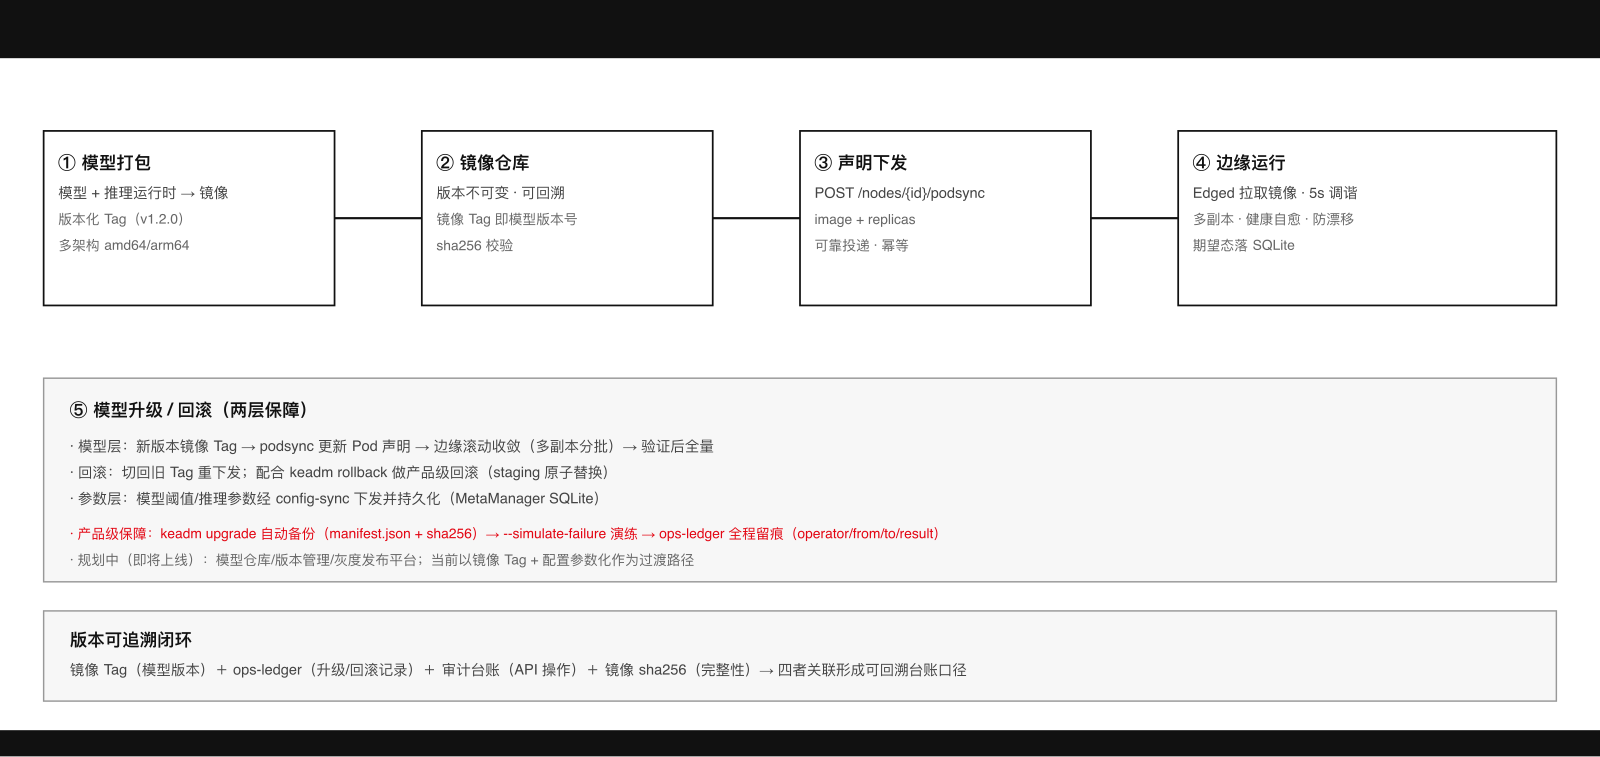
\includegraphics[width=0.94\textwidth]{../diagrams/scenario-model-mgmt.png}
  \caption{模型管理场景：镜像化模型分发链路}
  \label{fig:model-mgmt}
\end{figure}

\subsection{正式流程（v0.7.0，推荐）}

\textbf{模型部署 = 仓库注册 $\rightarrow$ 版本激活 $\rightarrow$ 灰度发布}（等效升级/回滚 = 新版本注册激活后再次发布 / rollback）：

\begin{lstlisting}
# ① 注册模型（模型名唯一；镜像实体在客户镜像仓库，平台登记 ref + sha256）
curl -X POST http://<cloudcore>:8080/api/v1/models \
  -H 'Content-Type: application/json' \
  -d '{"name":"defect-detector","description":"缺陷检测模型","type":"detection","metadata":{"owner":"qa-team"}}'

# ② 登记版本（"Tag 即版本"；初始 draft；sha256 必填）
curl -X POST http://<cloudcore>:8080/api/v1/models/defect-detector/versions \
  -d '{"version":"v1.2.0","mirror":"registry.example.com/edgeflow/models/defect-detector:v1.2.0","sha256":"sha256:9f86d081884c7d659a2feaa0c55ad015a3bf4f1b2b0b822cd15d6c15b0f00a08","sizeBytes":482344960,"archs":["amd64","arm64"],"metadata":{"threshold":"0.8"}}'

# ③ 激活版本（draft→active，自动降级旧 active；发布目标必须 active）
curl -X POST http://<cloudcore>:8080/api/v1/models/defect-detector/versions/v1.2.0/activate

# ④ 灰度发布（202 受理；先 1 台试点→小批→全量）
curl -X POST http://<cloudcore>:8080/api/v1/models/defect-detector/releases \
  -d '{"version":"v1.2.0","target":{"type":"percentage","percentage":25},"batchSize":2,"pauseBetween":30000,"failFast":true}'
# 白名单试点：{"version":"v1.2.0","target":{"type":"nodeIDs","nodeIDs":["edge-node-1"]},"batchSize":1,"pauseBetween":0,"failFast":true}

# ⑤ 跟踪 / 取消 / 回滚 / 台账
curl http://<cloudcore>:8080/api/v1/models/defect-detector/releases/<releaseID>    # perNode 汇总（summary 现算）
curl -X POST http://<cloudcore>:8080/api/v1/models/defect-detector/releases/<releaseID>/cancel
curl -X POST http://<cloudcore>:8080/api/v1/models/defect-detector/releases/<releaseID>/rollback   # 202 逆序回滚
curl http://<cloudcore>:8080/api/v1/models/defect-detector/deployments             # 版本—节点—时间台账
\end{lstlisting}

\begin{quote}
上述命令与字段均为示意用法，具体语法以产品文档（docs/API-SPEC.md §7）为准。
\end{quote}

\textbf{灰度运营建议}：

\begin{itemize}
  \item \textbf{节奏：先 1 台试点 $\rightarrow$ 小批 $\rightarrow$ 全量}。试点用白名单（1 台）验证镜像可用与推理结果；小批用 \texttt{batchSize=1\symbol{126}2 + pauseBetween $\ge$30s} 留观察窗口；验证通过后放大比例（25\% $\rightarrow$ 50\% $\rightarrow$ 100\%）或扩充白名单。
  \item \textbf{fail-fast 保持默认开（true）}：单节点失败立即中止，避免坏版本扩散；需要“收集全部节点失败情况”时再显式关闭。
  \item \textbf{回滚前置条件 = “该发布版本仍是模型当前 active 版本”}（未被新版本接管，否则 409）；回滚逆序批量执行、失败不回滚中止（能回多少回多少，perNode 明细可查）。
  \item \textbf{发布成功 $\neq$ 镜像可用}：平台下发的是声明（mirror ref），拉取发生在边缘；镜像仓库不可达/镜像损坏在边缘 PodStatus 暴露（CrashLoop 等）——发布前建议在试点节点确认 Pod Running。
  \item \textbf{耗时口径}：批内逐节点串行（每节点 2 次可靠下发，最坏 $\sim$10s+/节点超时）；batchSize 控制批粒度/暂停节奏，\textbf{不是并发度}；大 fleet 全量耗时 $\approx \Sigma$(单节点耗时) + $\Sigma$(pause)。
\end{itemize}

\subsection{产品升级灰度（keadm，双轨保留）}

keadm 升级分批（节点\textbf{软件}升级，与模型版本发布双轨并行）——\seqsplit{\texttt{keadm upgrade --batch-size/--pause-between}} 控制每批节点数与批间暂停，或 \seqsplit{\texttt{keadm batch --op=upgrade}} 按节点清单逐批执行（任一节点失败立即中止，fail-fast），实现“试点节点（1 台）$\rightarrow$ 小批节点 $\rightarrow$ 全量”的等效灰度：

\begin{lstlisting}
keadm upgrade --version <目标版本> --simulate-failure                        # 升级演练
keadm upgrade --version <目标版本>                                           # 正式升级
keadm upgrade --version <目标版本> --batch-size 5 --pause-between 30s        # 灰度分批：每批 5 台、批间暂停 30s
keadm batch --op=upgrade --file nodes.txt --version <目标版本> --batch-size 5 --pause-between 30s  # 按清单逐批升级（fail-fast）
\end{lstlisting}

\subsection{兼容路径（v0.1.0 时代过渡方案，仍可用）}

平台化能力（F41/F42）落地前，模型以“镜像 Tag + 手工声明”分发（能力上线后建议切换正式流程）：

\begin{enumerate}
  \item \textbf{模型打包}：模型文件与推理运行时打包为推理镜像，以镜像 Tag 承载模型版本（“镜像即模型、Tag 即版本”）；
  \item \textbf{镜像推送}：推送到客户既有镜像仓库（仓库承担模型存储职责）；
  \item \textbf{声明下发}：\seqsplit{\texttt{podsync}} 下发 Pod 声明（镜像版本 + 副本数）+ \seqsplit{\texttt{config-sync}} 下发模型参数（F31/F05）；
  \item \textbf{边缘执行}：Edged 声明式调谐拉取指定版本运行（F11/F12）；
  \item \textbf{版本升级}：新 Tag 构建推送后更新 Pod 声明，多副本分批滚动替换（F12）；
  \item \textbf{版本回滚}：Pod 声明恢复旧 Tag 重新下发，边缘自动收敛（应用级回滚）；产品级回滚走 \seqsplit{\texttt{keadm rollback}}（F39）；
  \item \textbf{版本追踪}：镜像 Tag + ops-ledger + 审计台账形成“版本—节点—时间”记录（正式流程下由部署影子 + perNode 台账取代）。
\end{enumerate}

\section{客户价值}

\begin{itemize}
  \item \textbf{版本可追踪}：模型仓库 + 部署影子 + 逐节点结果台账构成完整版本记录，任一节点当前模型版本与变更历史可查，问题可追溯（结果性描述）。
  \item \textbf{更新可控}：灰度发布按批推进、可暂停观察、可取消、可回滚，更新窗口与影响面受控，坏版本不扩散（fail-fast）。
  \item \textbf{回滚有保障}：逆序批量回滚到 prevActive（应用态），keadm rollback 覆盖产品态（双轨）；升级失败可快速恢复，敢升级、能回退。
  \item \textbf{边缘零改动}：发布/回滚复用既有 podsync/config-sync 链路，旧版 edgecore 直接可用，平台能力落地无边缘升级成本。
\end{itemize}